\documentclass[conference]{IEEEtran}
\IEEEoverridecommandlockouts
% The preceding line is only needed to identify funding in the first footnote. If that is unneeded, please comment it out.
\usepackage{cite}
\usepackage{amsmath,amssymb,amsfonts}
\usepackage{algorithmic}
\usepackage{graphicx}
\usepackage{textcomp}
\usepackage{xcolor}
\usepackage{lipsum,mathtools}
\usepackage{stmaryrd}
\usepackage[rightcaption]{sidecap}

\def\BibTeX{{\rm B\kern-.05em{\sc i\kern-.025em b}\kern-.08em
    T\kern-.1667em\lower.7ex\hbox{E}\kern-.125emX}}
\begin{document}

\title{Finite Difference Computations on GPU's with Applications to Wave Propagation Problems\\
}

\author{\IEEEauthorblockN{Toby Harvey}
\IEEEauthorblockA{\textit{University of Oregon, CIS 631}}}

\maketitle

\begin{abstract}
Partial differential equations (PDEs) , have been a staple technique for modeling physical phenomena within continuum since the advent of modern science and calculus. While these models have existed of over centuries, solving them has remained somewhat elusive. Deriving analytic solutions seems only possible for "toy" problems and the computational expense of solving them numerically has been a serious bottleneck in producing solutions to physically realistic complex problem. In recent years computer hardware has become powerful enough that many problems thought  to complex to solve are now computationally viable. Most numerical methods for solving PDEs  boil down to doing lots of matrix and vector multiplication. Graphics Processing Units (GPUs) are highly optimized for these kinds of operations on the hardware level and therefore are an enticing choice for PDE models. In this paper we will investigate the difficulties in solving PDEs using the finite difference (FD) method on GPUs. We will categorize these difficulties, and survey some techniques that have already been implemented in FD GPU codes.
\end{abstract}

\section{Introduction}
In many scientific domains partial differential equations are used to model the movement of important quantities such as concentration, temperature, pressure, displacement, etc. through spatial and temporal domains. The main three examples being the heat equation (heat flow), wave equation (wave propagation), and Poisson's equation (multiple applications to equilibrium situations). The goal of creating these models is to solve the PDE by finding a function of the two, three or four independent variables (space and time) for the quantity of interest so that the scientist can make predictions about physical phenomena or help inform engineers. While many analytic solutions on simple domains with simple boundary conditions and homogeneous material properties exist for the above equations, in practice scientists are interested in problems formulated on complex physically realistic domains with potentially nonlinear boundary and interface conditions for which known solutions do not exist. FD approximations are one numerical method of solving for PDE's that are widely used. FDs do not attempt to uncover a underlying function that satisfies the PDE but instead discretize the domain of the problem into a set of nodes on which the practitioner seeks a solution. As the domain is refined with an increasing number of nodes, FD methods are known to converge to a solution. In the past FD schemes have received criticism for not being able to  handle complex geometries naturally. Although not directly built into schemes like finite volume (FV), or finite element (FE), finite difference can also handle complex geometries through coordinate transformations between computational and physical space using methods such as transfinite interpolation \cite{LeVeque}. FD methods are also significantly simpler in their theoretical derivations than FV and FE methods, also increasing their appeal.

There are multiple different ways in which FD methods can become computationally expensive:  Specific scientific applications may require large domain sizes; Accurate solutions may require large  numbers of nodes or  finite difference stencils that use many nearby nodes to estimate derivatives at each node.  Using the parallelism in FD methods then becomes important for solving physically realistic problem, and therefore finding the best mappings between FD operators and GPU architecture and software constructs is also important.

This survey will attempt to do present previous strategies taken to parallelize both first order FD operators, discrete laplacian operators, and other FD operators relevant to wave propagation problems over 3D large spatial domains. In II. we will present a background overview of the finite difference method. In III. we will attempt to characterize the difficulties involved with writing FD code on a GPU, and then in IV. We will present different methods that have been taken to solve these issues in previous GPU and multi-GPU implementations.

\section{Background}

As an example of a finite difference method consider solving the wave equation in 2D. We won't consider any boundary conditions (which would exist in a real application problem). We want to find a function $u(x, y, t)$ such that:
\begin{align}
&\frac{\partial^2 u}{\partial t^2} = c^2\left(\frac{\partial^2u}{\partial x^2} + \frac{\partial^2 u}{\partial y^2}\right) \quad (x,y) \in [0, 1] \times [0,1], t \in [0,T]\\
&u(x, y, 0) = f(x,y), \quad (x,y) \in [0, 1] \times [0,1]
\end{align}
Where $c$ is the wave speed. The FD method discretizes the domain and produces an approximation of the solution at every node. Paritioning the domain into $N$ equidistant grid points in both spatial directions and $M$ equidistant points in the time domain we get:
\begin{align*}
&x_i = ih, \quad i = 0,1,...N, \quad h = \frac{1}{N-1}\\
&y_j = jh, \quad j = 0,1,...N\\
&t_l = lk, \quad l = 0,1,...M, \quad k = \frac{T}{M-1}\\
\end{align*}
The discrete approximation of $u$ and grid point $(x_i, y_j, t_l)$ is then denoted $u^l_{i,j}$. The FD method uses the weighted sum of neighboring $u$'s to approximate derivatives of $u$ at a single grid point. This can be more rigorously derived with the Taylor series, and error bounds can also be produced, but we skip this as we are focused on implementing these computations on the GPU and just consider the formulas for each derivative in (1). A centered difference in space can be computed by considering the difference of two first neighboring first derivatives. For example in the x direction (but this also applies in the y direction:
\begin{align}
    \nonumber&\frac{\partial u}{\partial x}\bigg\rvert_{x=x_i} \approx \frac{u^l_{i,j} - u^l_{i-1,j}}{h}\\
    \nonumber&\frac{\partial^2u}{\partial x^2}\bigg\rvert_{x=x_i}\approx\\ \nonumber&\frac{\frac{\partial u}{\partial x}\big\rvert_{x=x_i+1} - \frac{\partial u}{\partial x}\big\rvert_{x=x_i}}{h} \approx\\
    &\frac{u^l_{i+1,j} - 2u^l_{i,j} + u^l_{i-1,j}}{h^2}\ = \\
    & \delta_x u^l_{i,j}
\end{align}
Combining this approximation of the second $x$ derivative with the $y$ derivative we get an approximation of the laplacian operator (LHS of the wave equation):
\begin{align}
    \Delta u^l_{i,j} \approx \frac{u^l_{i+1,j} + u^l_{i-1,j} + u^l_{i,j+1} + u^l_{i,j-1} - 4u^l_{i,j} }{h^2}
\end{align}

This computation relies on the value at the node itself an a the neighboring nodes to each side of it. The term $k$ length stencil (not to be confused with $k$ length time-step) is used to denote the number of nodes in a given direction the approximation takes. In our case only 3. Using Taylor series we can show that by increasing the stencil length the order of accuracy of the approximation increases. In a much more general setting applying a centered finite difference operator in 2D takes the form:
\begin{align}
    \partial u^l_{i,j} \approx \sum_{s=1}^{\frac{k}{2}} c^x_s(u^l_{i-s,j} + u^l_{i+s,j}) + c^y_s(u^l_{i,j-s} + u^l_{i,j+s})
\end{align}


\subsection{Explicit Method}

Lastly the time domain can be discretized in the same way space was in (4), which leads to an explicit scheme where explicit means all data is known except for a single value of $u$ which is computed with the known data:
\begin{align}
&u^{l+1}_{i,j} = 2 u^l_{i,j} - u^{l-1}_{i,j} + c^2k^2\Delta u^l_{i,j}
\end{align}

To complete the method we sample the initial condition (2) at all spatial grid points, and use that as our first data in (6), and continue to march forward in time till $T$. This method can be implemented by stacking one axis, say $y$ in $u$, and doing a matrix multiplication at every time-step, although in practice this may be slower than a matrix free version.

\subsection{Implicit Method}

When we apply boundary conditions to our problem, the computations near $i=0$, $i=N$, $j=0$, $j=N$  change to impose these conditions, and (6) looks slightly more complicated. In many scientific applications the addition of certain boundary conditions, or highly varying material parameters like wave speed leads to numerical stiffness, i.e. a prohibitively small time-step needs to be taken in order to maintain numerical stability\cite{Lambert}. Analysis can be done to show that implicit time stepping methods are unconditionally stable regardless of time step, and are therefore implementing them on GPUs is also worth considering. We can make our method implicit by making our time derivative equal to the average of spatial derivatives at a previous and future time step:
\begin{align}
&u^{l+1}_{i,j} - \frac{c^2}{2}(\delta_x u^{l+1}_{i,j} + \delta_y u^{l+1}_{i,j}) = \\
\nonumber&2 u^l_{i,j} - u^{l-1}_{i,j} + \frac{k^2c^2}{2}(\delta_x  u^{l-1}_{i,j} + \delta_y u^{l-1}_{i,j})
\end{align}

Now a linear system must be solved  to update $u$ to the next time step. The computations associated with a linear system solve can be significantly different than solving the explicit scheme on a GPU, and therefore we treat implicit and explicit schemes in difference sections from now on. Upon factoring $u^{l}_{i,j}$ out in the LHS of (7) and stacking the vector in one spatial direction (7) can be reduced to a system $Au = b$ where $b$ are the known data. $A$ is sparse, highly ordered, and usually symmetric, meaning that the problem of porting a finite difference method to the GPU really becomes one of optimizing methods for solving sparse highly ordered systems.

\section{Characterization of difficulties}

Porting FD methods to the GPU can take different forms. For time varying equations, the entire discretization in both space and time can be coded from scratch on the GPU such as in (6) or (7). Alternatively, just the spatial discretization can be done, resulting in a matrix equation $\frac{\partial^c u}{\partial t^c} = A\boldsymbol{u}$ which can then be passed to an ordinary differential equation (ODE) solver such as RK4 to be time integrated either implicitly or explicitly. Libraries such as Julia's differentialequations.jl  already have many GPU optimized time-stepping implementations\cite{diff}. In the rest of this paper, we examine situations in which spatial and time discretizations have already been done. We categorize the difficulties of writing good FD code on the GPU into $n$ sections/problems:

\subsubsection{FDs are memory bound}
Taking for example equation (5) to compute the differential operator at a single grid point $k-1$ reads need to be made in each of $n$ dimensions plus the previous value at the current node for $n(k-1) + 1$ reads, and single write is needed. Whereas the number of computations done on the data is relatively small and can be done very fast, demonstrating that FD methods are inherently memory bound. Zhou et al.\cite{Zhou1} did analysis of a 3D FD earthquake simulation code and found that their two finite difference kernels average to have a Flops/Bytes ratio of 0.508. While this ratio can be lowered using good memory access practices, FD operators are ultimately intrinsically bandwidth bound just by the computations associated with them.

\subsubsection{Memory Coalescing}

On the GPU global memory is accessed by warp (32 threads) in chunks of 32, 64 or 128 bytes. If memory access is scattered over an array in device memory, many memory accesses will need to be made to read in data. Since global memory accesses a relatively low bandwidth, it is important that threads in a warp access coalesced memory. In three dimensional FD computations the order in which $u$ is stored by dimension will have an effect on memory access patterns, and ideally the dimension in which the most computations are done is mapped to the fastest index \cite{Harris}.

\subsubsection{Utilization of different types of memory}

On GPUs different types of memory have different associated bandwidths. Global memory usually has low bandwidth. Each thread block has a shared memory bank which has significantly higher bandwidth. Data can be stored locally in registers, and lastly there is read only textured memory which is faster than Global memory. Where previously computed data is stored when a warp accesses it will directly affect the speed at which that warp can commute a FD computation\cite{Harris}.


\subsubsection{Domain Decomposition}

The domain sizes are usually very large, or the cell sizes are very small, in FD codes one would wish to run on a GPU. Additionally models in 3D or more dimensions are of interest, and each dimension greatly increases the number of computations per node. Thus the mapping of the physical domain to the thread geometry becomes important. For instance, deciding what sections of the mesh will be loaded into shared memory, how many nodes a single thread will operate on in a given time-step, and the dimension of thread blocks become important\cite{Michea}.

\begin{figure}[h]
\caption{Halos for 2D and 3D threadblock mapping as seen in \cite{Michea}}
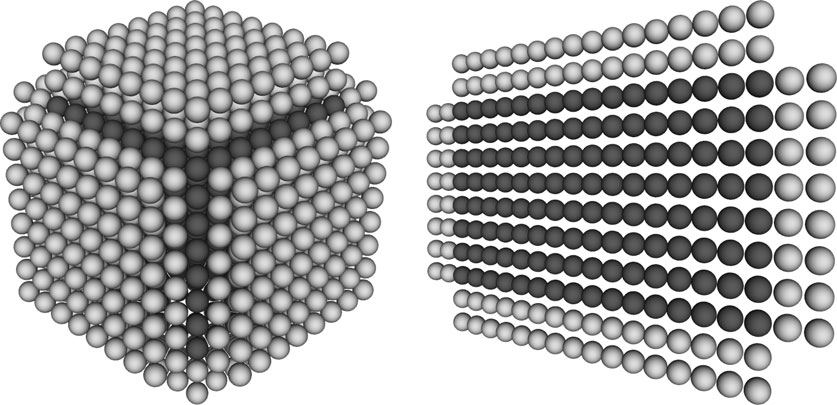
\includegraphics[scale=.25]{halos.png}
\end{figure}
\section{Survey of Past GPU Implementations}

\subsection{Single GPU Explicit Wave Propagation Problems}

In all of the following implementations, the authors map a single thread to either single spatial nodes, or a single line of nodes in one spatial direction, and then have that thread calculate the FD computation at a single node or the line of nodes. In order for a thread to compute a finite difference, it needs access to the point it is mapped to and also its $\frac{k}{2}$ neighbors. A naive approach to mapping in 3D physical domain is to use 3D dimensional thread blocks so that each thread is indexed by $(i,j,k)$ (here $k$ indexes the 3rd spatial dimension and is not the temporal step size as it was before) so that the volume is decomposed into sub-volumes on which computations take place\cite{Michea}. Hamilton et al.\cite{Hamilton} take this approach in a kernel design for room acoustics modeling. They use a complicated FD stencil that is staggered such that neighboring threads access a significant number of independent neighbors from each other to approximate a discrete Laplacian. The data that each thread in a block needs to access is therefore not all reused by neighboring threads, and the authors elect to not use any shared memory. One disadvantage to this method, that the authors note, is that the points of both stencils need to be read into local memory in order to insure memory coalescing, and a conditional must be issued in the kernel to decide which stencil is used. They observe a speed-up of 48X between a serial code on an Xeon E5-2620, and the GPU code on a Tesla K20. If shared memory is used, then, at boundaries of the each sub-volume, a thread block will need access to memory outside of the volume. This is is commonly refereed to as a halo region. Both Micikevicius\cite{Micikevicius}, and Michea et al.\cite{Michea} consider using a 3D thread indexing scheme, but settle on 2D schemes. In Michea et al.'s\cite{Michea} analysis, they assume each thread will load its own physical value into shared memory and, thus, within a block each thread will have access to its neighbors in shared memory. The additional halo region will also be loaded into shared memory. They note that an intuitive reason for using 3D thread blocks is that with large enough blocks the ratio of grid points to halo size becomes quite small. The problem is that, in practice, shared memory banks are not large enough on GPUs right now to store the data needed for this ratio to be small. Micikevicius\cite{Micikevicius} makes a similar assertion, and both opt for methods that tile 2D slices of the 3D physical domain and then iterate over the unrepresented dimension within the tile. The 2D tiling approach appears to be a common technique among implementations, and has quite a few advantages. With 2D tiles, the halo region reduces to a half stencil width outline around the 2D region, and half stencil width number of planes on each side of the tile for the unrepresented dimension. Micikevicius\cite{Micikevicius} uses the ratio of number of nodes accessed to number of nodes processed in a thread block as a metric of performance and notes that in the 2D scheme increasing the length of the block dimensions will minimize this ratio -- the same assertion that Michea et al. makes, but for the 2D case. Both these papers employ the same marching technique so that a single thread will compute all the FDs in the "off direction" as follows:


\begin{itemize}
    \item Load each data point a thread is responsible for into shared memory.
    \item Separately load in the half region in the "on" directions into shared memory.
    \item Load the $k-1$ elements needed in the "off" direction computation into local memory for each thread.
    \item compute the FD operator
    \item iterate in the "off" direction by shifting all of the elements in registers down 1 for each thread in the block, and repeat
    \end{itemize}


\begin{figure}[h]
\caption{Data usage around a group of thread iterating in Z direction as seen in \cite{Micikevicius}}
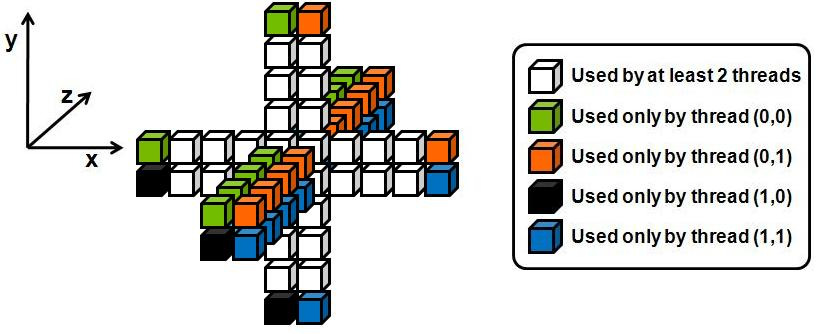
\includegraphics[scale=.25]{data2d.png}
\end{figure}


This technique seems to out perform a 3D thread block scheme for normal FD stencils. Michea et al.\cite{Michea} finds that there is about twice as few memory accesses per grid point with fourth order operators, and 16 by 8 thread blocks, versus fourth order operators, and 5 by 5 by 5 thread blocks. While this may be a good mapping from the physical domain to threads, we have not addressed memory coalescing or usage of textured memory. Zhou et al.\cite{Zhou1} in their 3D earthquake simulator also use a 2D thread block approach. They discuss how they insure memory coalescing by noting that, if the domain is stored in a 3 dimensional array in CUDA of $x$, then $y$ then $z$ the fastest dimension will be $z$, then $y$ meaning that each thread-block should be in the $yz$ plane of the physical domain, and iterate through the x plane. In performance tests they found that blocks in the $yz$ plane out-perform blocks in the $xy$ plane by about half the time per single iteration over the spatial domain. Secondly, in order to make sure that memory is aligned in blocks of 32 bytes accessed by each warp individually, padding of zeros is added to the ends of the Z dimension so that access is coalesced.
Lastly as mentioned in \cite{Harris} taking advantage of the textured memory to store read only data should increase performance by a bit. This is optimal memory to store the difference stencil coefficients in and any material parameters associated with the equations. In the case of spatial varying material properties this could account for a lot of data and would probably see substantial speed up by being placed in constant memory.

\subsection{Single GPU Implicit Implementation}

In implicit time-stepping methods, a sparse linear system must be solved. There are many different algorithms for such systems dependent on the structure of the system the stencil produces, and solving these systems is a whole subject onto itself so we only briefly touch on it. As a good example the stencil for a 1d second derived, as in equation (3) which produces a symmetric tridiagonal matrix, can be efficiently solved with the parallel cyclic reduction (PCR) algorithm. PCR uses the fact that each equation within the system has identical coefficients, but is just shifted one set of variables over, starting with all the even numbered. The equation above and below it can be combine into a new system with exactly half the unknowns at each iteration all of even index and this operation can be performed until all even-numbered variables can be solved for and a back substitution phase applied. Giles et al.\cite{Giles} use the PCR algorithm in the context of solving the 1D Black-Scholes equation, but the 1d Laplacian produces a similar tridiagonal system. In their implementation, each warp solves a different 1D problem, and each thread handles multiple nodes. The 2D Laplacian (5) produces a block tri-diagonal matrix, which means PCR can be used on it as well:

$$
\begin{bmatrix}
A & I & ... & & & \\
I & A & I & ... & & & \\
  & I & A & I & ... & & & \\
  & \vdots & \vdots & \vdots & \vdots & & & \\
  &   &   &   & & I & A & I & \\
  &   &   &   & & & I & A \\
\end{bmatrix}
A = \begin{bmatrix}
  -4 & 1 & ... & & & \\
  1 & -4 & 1 & ... & & & \\
  & 1 & -4 & 1 & ... & & & \\
  & \vdots & \vdots & \vdots & \vdots & & & \\
  &   &   &   & & 1 & -4 & 1 & \\
  &   &   &   & & & 1 & -4 \\
\end{bmatrix}
$$

The mapping of systems to warp and multiple equations to thread in Giles et al.\cite{Giles} will not work for such a big system, hence we investigate the implementation of PCR by Zhang et al.\cite{Zhang} They instead map systems to be solved to thread blocks, and equations to individual threads. For each block they load the three diagonals of the matrix and the right hand side into shared memory. Since shared memory can only store up to 512 equations, single blocks can only solve small systems. In the reduction part of the algorithm they half the number active threads each time, and than double in the back substitute part. This GPU implementation would better than the Giles et al.\cite{Giles} implementation for a PDE problem but again could not solve large enough systems for a real world application. Zhang et al.\cite{Zhang} do implement a solver that uses pure global memory and no shared memory but see a 3X performance degradation.

\subsection{Multi-GPU explicit Wave propagation Problems}

For some seismic and acoustic wave simulations the global memory of a single GPU is still not enough, and therefore multiple GPU implementations are used. In the implementation I survey each GPU will communicate relevant data to each other GPU through a message passing interface (MPI). In the same way that thread blocks needed to load halo regions in the single GPU implementations into shared memory to do computations that involve nodes outside of the block domain, when we partition the domain into sections for individual GPUs the computations at the boundary nodes of the GPU will require that values from nodes in another GPU are passed to them\cite{Okamoto}. These nodes are refereed to as ghost nodes. When decomposing the physical domain to different GPUs the effect of ghost nodes needs to be considered. Zhou et al.\cite{Zhou} continues their work by creating a scheme in which they link their single GPU implementation between a network of GPUs. The domain is partitioned in the $xy$ plane with a single GPU assigned to a cell. Each GPU will compute all of the nodes within the partition and along the $z$ axis. Then each individual GPU is partitioned in the same way that was presented in \cite{Zhou1}. This leaves each GPU with a plane of ghost nodes in the $z$ direction on the east, west, north, and south (if it isn't a "boundary GPU"). This mapping allows a single GPU to iterate through the entire $z$ direction which was shown to be efficient in \cite{Zhou1}. In contrast Okamoto et al. \cite{Okamoto} map each GPU to a 3D cell within the domain instead of a column. They note that communication time between GPUs will decrease with increasing number of partitions, and in schemes where the domain can only be extended in one direction the size of the plane of ghost nodes won't decrease, and hence are not scalable. Regardless of the mapping of the physical domain to each GPU, the order of communication between GPUs and the overlapping scheme of computation with communication are important for performance. If a GPU receives old data in its ghost cells this will obviously decrease accuracy, and hence the order of passing must be addressed. This is done in both implementations by each scheduling an passing order for each block i.e. first send/recv east and west then north and sound. Secondly, there are performance benefits to optimizing the message passing scheme by overlapping it with the GPU computations as the message passing will have the highest latency. Zho et al.\cite{Zhou} does this in a fairly complex scheme which takes advantage of the dependencies that stress computations have on velocity computations an visa versa in the elastic wave equation (see figure 3).


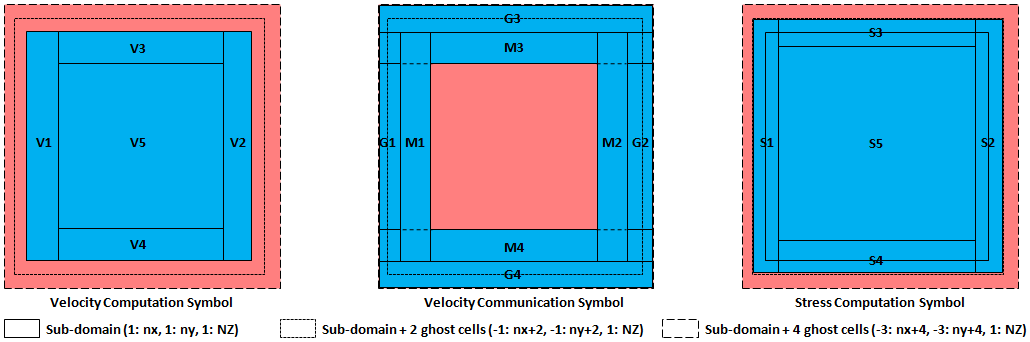
\includegraphics[scale=.25]{passing.png}
\begin{figure}[h]
\caption{Compuation and Message passing scheme for overlap in GPU cluster as in \cite{Zhou}.}
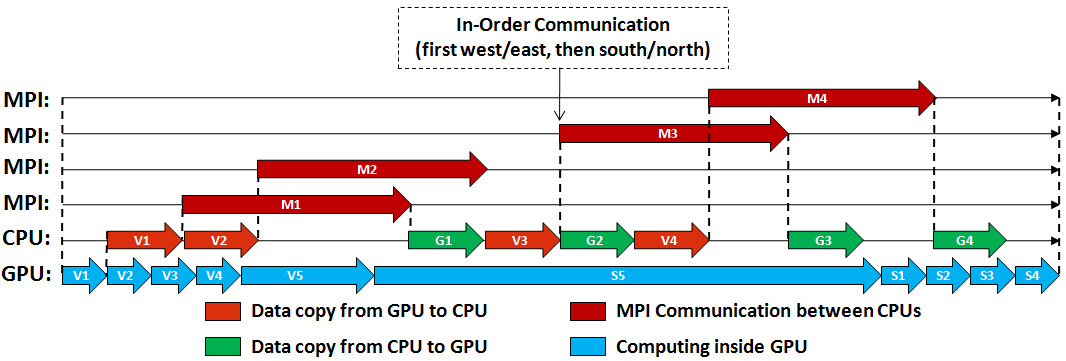
\includegraphics[scale=.25]{passing2.png}
\end{figure}

\section{Conclusion}
In this work we have investigated some FD methods for solving PDEs on GPUs. These methods include both explicit and implicit time-stepping schemes, and single and multi GPU architectures. Although this seems like it would be a highly researched area from a scientific perceptive, I was struck by the similarity of most explicit implementations. This could be for one of two reasons. Either these similar implementations are the optimal implementation, or less work as been done in this field that I expected and more investigation could lead to much faster codes. Lastly, all of these methods assumed the GPU programmer can make reasonable decisions in attempting to map the physical domain and computations onto the GPU hardware. While this seems like a completely reasonable strategy I would be interested if mathematical optimization problems are ever formulated to solve this mapping for the GPU programmer.


\begin{thebibliography}{12}

\bibitem{Abdelkhalek}
R. Abdelkhalek, H. Calendra, O. Coulaud, G. Latu, and J. Roman, ''Fast Seismic Modeling and Reverse Time Migration on a GPU Cluster,'' The 2009 High Performance Computing & Simulation, 2009.

\bibitem{Cohen}
S. Cohen, ''Cyclic Reduction,'' 1994.

\bibitem{diff}
DifferentialEquations.jl, https://diffeq.sciml.ai/v2.0/.

\bibitem{Giles}
M. Giles, E. Lászlo, I. Reguly, J. Appleyard, and J. Demouth, ''GPU Implementation of Finite Difference Solvers,'' 2014 Seventh Workshop on High Performance Computational Finance, November 2014.

\bibitem{Hamilton}
B. Hamilton, C. J. Webb, "Room Acoustics Modelling Using GPU-Accelerated Finite Difference and Finite Volume Methods on a Face-Centered Cubic Grid,'' 16th Int. Conference on Digital Audio Effects, 2013.

\bibitem{Harris}
M. Harris, 'Finite Difference Methods in CUDA C/C++, Part 1,' Nvidia Developer Blog, 4 March 2013, available at: https://developer.nvidia.com/blog/finite-difference-methods-cuda-cc-part-1 (accessed 1 November, 2020).

\bibitem{Lambert}
J. D. Lambert, Numerical Methods for Ordinary Differential Systems: The Initial Value Problem. 1991. 

\bibitem{LeVeque}
R. J. LeVeque, Finite Difference Methods for Ordinary and Partial Differential Equations: Steady-State an Time-Dependent Problems. University of Washington: Seattle, 2007.

\bibitem{Michea}
D. Michéa, D. Komatitsch, ''Accelerating a three-dimensional finite-difference wave propagation code using GPU graphics cards,'' Geophysical Journal International, vol. 182, pp. 389--402, July 2010.

\bibitem{Micikevicius}
P. Micikevicius, ''3D finite difference computation on GPUs using CUDA,'' in Proceedings of 2nd Workshop on General Purpose Processing on Graphics Processing Units, pp. 79--84, 2009.

\bibitem{Okamoto}
T. Okamoto, H. Takenaka, T, Nakamura, and T. Aoki, ''Accelerating Large-Scale Simulation of Seismic Wave Propagation by Multi-GPUs and Three-Dimensional Domain Decomposition,'' Lecture Notes in Earth System Sciences, pp. 375--389, January 2013.

\bibitem{Strikwerda}
J. C. Strikwerda, Finite Difference Schemes and Partial Difference Equations, 2nd ed. University of Wisconsin: Madison, 2004.

\bibitem{Zhang}
Y. Zhang, J. Cohen, J. Owens, ''Fast tridiagonal solvers on the GPU,'' 15th ACM SIGPLAN Symposium on Principles and Practice of Parallel Programming, 2010.

\bibitem{Zhou}
J. Zhou, Y. Ciu, E. Poyraz, D. J. Choi, and C. C. Guest, ''Multi-GPU Implementation of a 3D Finite Difference Time Domain Earthquake Code on Heterogeneous Supercomputers,'' Procedia Computer Science, vol. 18, pp. 1255--1264, 2013.

\bibitem{Zhou1}
J. Zhou, D. Unat, D. J. Choi, C. C. Guest, Y. Cui, ''Hands-on Performance Tuning of 3D Finite Difference Earthquake Simulation on CPU Fermi Chipset,''Procedia Computer Science, vol. 9, pp. 976--985, 2012.

\end{thebibliography}

\end{document}
